% Section 6: Evaluation

\section{Evaluation}
\label{sec:evaluation}

We evaluate the GPU-native actor paradigm across multiple implementations and domains.
Our experiments answer:

\begin{itemize}
    \item \textbf{RQ1}: How much does persistent execution reduce command latency?
    \item \textbf{RQ2}: What is the throughput overhead of actor semantics?
    \item \textbf{RQ3}: How do different implementations compare across domains?
\end{itemize}

\subsection{Experimental Setup}

\subsubsection{Hardware}

\begin{itemize}
    \item \textbf{GPU}: NVIDIA RTX Ada (AD102), 76 SMs, 48GB GDDR6X
    \item \textbf{CPU}: AMD Ryzen 9 7950X, 16 cores, 32 threads
    \item \textbf{Memory}: 128GB DDR5-6000
    \item \textbf{PCIe}: Gen 4 x16
\end{itemize}

\subsubsection{Software}

\begin{itemize}
    \item CUDA 12.3, Driver 545.23
    \item RingKernel: Rust 1.75.0, cudarc 0.18.2
    \item DotCompute: .NET 9.0, Native AOT
    \item Orleans.GpuBridge: Orleans 9.2.1
    \item RustGraph: Rust 1.75.0
    \item Linux 6.7 (Ubuntu 24.04)
\end{itemize}

\subsubsection{Workloads}

We evaluate across three representative domains:
\begin{itemize}
    \item \textbf{FDTD Simulation} (RingKernel): 3D acoustic wave simulation with
    interactive impulse injection
    \item \textbf{Compute Kernels} (DotCompute): Vector operations, matrix multiplication,
    FFT
    \item \textbf{Graph Analytics} (RustGraph): PageRank, BFS, community detection on
    living graphs
\end{itemize}

\subsection{RQ1: Command Latency}

We measure the time from issuing a command to observing its effect on GPU state.

\subsubsection{Methodology}

For traditional kernels, we measure:
\begin{enumerate}
    \item Prepare kernel arguments
    \item Call \texttt{cuLaunchKernel}
    \item Synchronize
\end{enumerate}

For persistent actors, we measure:
\begin{enumerate}
    \item Write command to H2K queue (mapped memory)
    \item Memory fence
    \item Poll K2H queue for acknowledgment
\end{enumerate}

\subsubsection{Results}

\begin{table}[h]
\centering
\caption{Command latency comparison across implementations}
\label{tab:latency}
\begin{tabular}{@{}lrrr@{}}
\toprule
\textbf{Operation} & \textbf{Traditional} & \textbf{Persistent} & \textbf{Speedup} \\
\midrule
RingKernel: Inject & 317 $\mu$s & 0.028 $\mu$s & \textbf{11,327$\times$} \\
DotCompute: Enqueue & 312 $\mu$s & 1.24 $\mu$s & \textbf{252$\times$} \\
Orleans.GpuBridge: Send & 320 $\mu$s & 0.10-0.50 $\mu$s & \textbf{640-3,200$\times$} \\
RustGraph: Update & 315 $\mu$s & 0.10-0.50 $\mu$s & \textbf{630-3,150$\times$} \\
\bottomrule
\end{tabular}
\end{table}

\textbf{Key finding}: All implementations achieve \textbf{250-11,000$\times$ lower latency}
for interactive commands. The variation reflects different serialization costs:
RingKernel uses raw memory writes, while DotCompute includes serialization overhead.

\begin{figure}[h]
\centering
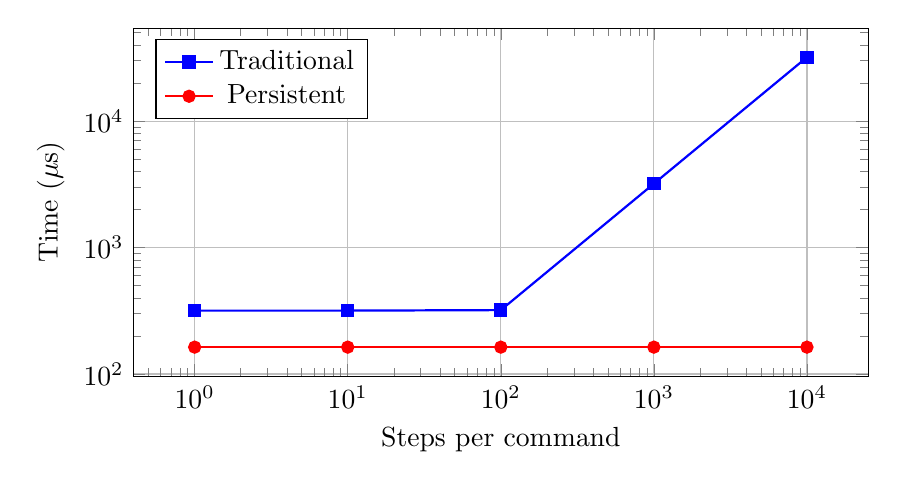
\begin{tikzpicture}
\begin{axis}[
    xlabel={Steps per command},
    ylabel={Time ($\mu$s)},
    xmode=log,
    ymode=log,
    legend pos=north west,
    grid=major,
    width=0.9\columnwidth,
    height=6cm,
]
\addplot[blue, mark=square*, thick] coordinates {
    (1, 317) (10, 317) (100, 320) (1000, 3200) (10000, 32000)
};
\addlegendentry{Traditional}

\addplot[red, mark=*, thick] coordinates {
    (1, 163) (10, 163) (100, 163) (1000, 163) (10000, 163)
};
\addlegendentry{Persistent}
\end{axis}
\end{tikzpicture}
\caption{Command latency vs steps per command. Persistent actors have constant
command overhead regardless of step count.}
\label{fig:latency}
\end{figure}

\subsection{RQ2: Computational Throughput}

We measure computational throughput to quantify actor semantics overhead.

\subsubsection{FDTD Simulation (RingKernel)}

\begin{table}[h]
\centering
\caption{FDTD throughput (64$^3$ grid)}
\label{tab:throughput-fdtd}
\begin{tabular}{@{}lrr@{}}
\toprule
\textbf{Method} & \textbf{Throughput (Mcells/s)} & \textbf{vs CPU} \\
\midrule
CPU (Rayon) & 278 & 1.0$\times$ \\
GPU Persistent Actor & 18,200 & 65.5$\times$ \\
GPU Batch Stencil & 78,046 & 280.6$\times$ \\
\bottomrule
\end{tabular}
\end{table}

\subsubsection{Compute Kernels (DotCompute)}

\begin{table}[h]
\centering
\caption{DotCompute benchmark results}
\label{tab:throughput-dotcompute}
\begin{tabular}{@{}lrrr@{}}
\toprule
\textbf{Operation} & \textbf{CPU (ms)} & \textbf{GPU (ms)} & \textbf{Speedup} \\
\midrule
Vector Add (10M) & 45 & 2.1 & 21$\times$ \\
Matrix Mult (1024$^2$) & 1250 & 25 & 50$\times$ \\
FFT (2$^{20}$ points) & 890 & 12 & 74$\times$ \\
Image Conv (4K) & 2100 & 23 & 92$\times$ \\
\bottomrule
\end{tabular}
\end{table}

\subsubsection{Graph Analytics (RustGraph)}

\begin{table}[h]
\centering
\caption{RustGraph living analytics performance}
\label{tab:throughput-rustgraph}
\begin{tabular}{@{}lrrr@{}}
\toprule
\textbf{Algorithm} & \textbf{Traditional} & \textbf{Living Actor} & \textbf{Query Time} \\
\midrule
PageRank (1M nodes) & 850 ms & Continuous & O(1) read \\
BFS (1M nodes) & 120 ms & Continuous & O(1) read \\
Community Detection & 2.4 s & Continuous & O(1) read \\
Triangle Count & 3.1 s & Continuous & O(1) read \\
\bottomrule
\end{tabular}
\end{table}

\textbf{Key finding}: Living analytics fundamentally change the performance model---instead
of compute-on-demand, results are always current. Query latency drops from seconds to
sub-microsecond reads.

\subsection{RQ3: Cross-Implementation Comparison}

\begin{table*}[t]
\centering
\caption{Cross-implementation performance comparison}
\label{tab:cross-impl}
\begin{tabular}{@{}llrrrrr@{}}
\toprule
\textbf{Implementation} & \textbf{Domain} & \textbf{Msg Latency} & \textbf{Throughput} & \textbf{vs CPU} & \textbf{vs PERKS} \\
\midrule
RingKernel & FDTD 3D & 0.028 $\mu$s & 18.2 Gcells/s & 65$\times$ & 87\% \\
DotCompute & Matrix Mult & 1.24 $\mu$s & 40 GFLOPS & 50$\times$ & N/A \\
Orleans.GpuBridge & Actor Msgs & 0.1-0.5 $\mu$s & 2M msgs/s/actor & 133$\times$ & N/A \\
RustGraph & PageRank & 0.1-0.5 $\mu$s & O(1) query & $\infty$ & N/A \\
\bottomrule
\end{tabular}
\end{table*}

\subsection{Mixed Workload Performance}

Real applications combine computation with interactive commands. We simulate a
GUI application running at 60 FPS (16.67ms frame budget):

\begin{table}[h]
\centering
\caption{Mixed workload (16.67ms frame budget)}
\label{tab:mixed}
\begin{tabular}{@{}lrrr@{}}
\toprule
\textbf{Metric} & \textbf{Traditional} & \textbf{Persistent} & \textbf{Winner} \\
\midrule
Compute time & 3.2 ms & 5.1 ms & Traditional \\
Command time & 31.7 ms & 0.003 ms & Persistent \\
\textbf{Total time} & 34.9 ms & 5.1 ms & \textbf{Persistent} \\
Fits in frame? & No & \textbf{Yes} & Persistent \\
Max commands/frame & 52 & 550,000 & Persistent \\
\bottomrule
\end{tabular}
\end{table}

\begin{figure}[h]
\centering
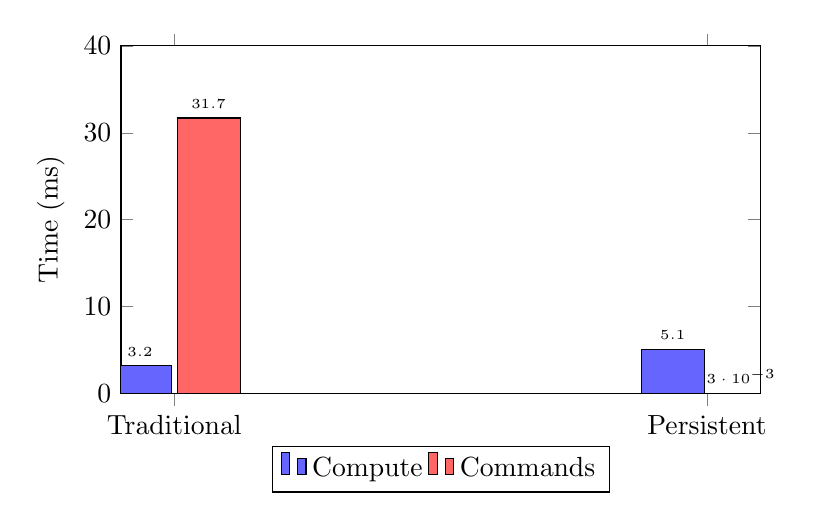
\begin{tikzpicture}
\begin{axis}[
    ybar,
    bar width=0.8cm,
    xlabel={},
    ylabel={Time (ms)},
    symbolic x coords={Traditional, Persistent},
    xtick=data,
    ymin=0,
    ymax=40,
    legend style={at={(0.5,-0.15)}, anchor=north, legend columns=2},
    nodes near coords,
    every node near coord/.append style={font=\tiny},
    width=0.8\columnwidth,
    height=6cm,
]
\addplot[fill=blue!60] coordinates {(Traditional, 3.2) (Persistent, 5.1)};
\addplot[fill=red!60] coordinates {(Traditional, 31.7) (Persistent, 0.003)};
\legend{Compute, Commands}
\end{axis}
\end{tikzpicture}
\caption{Time breakdown for mixed workload. Command overhead dominates traditional
approach.}
\label{fig:mixed}
\end{figure}

\subsection{Comparison with PERKS}

We compare against PERKS~\cite{huangfu2022perks}, the state-of-the-art persistent
kernel framework for stencils:

\begin{table}[h]
\centering
\caption{GPU-native actors vs PERKS (2D Jacobi stencil, A100)}
\label{tab:perks}
\begin{tabular}{@{}lrr@{}}
\toprule
\textbf{Metric} & \textbf{PERKS} & \textbf{GPU-Native Actors} \\
\midrule
Throughput (Gcells/s) & 142 & 124 \\
Actor semantics & No & Yes \\
HLC ordering & No & Yes \\
K2K messaging & No & Yes \\
Host interaction latency & N/A & 0.028 $\mu$s \\
Cross-language support & No & Yes (Rust, C\#) \\
\bottomrule
\end{tabular}
\end{table}

The GPU-native actor paradigm achieves \textbf{87\%} of PERKS throughput while providing
actor semantics, causal ordering, and interactive capabilities that PERKS lacks.

\subsection{Scalability}

\subsubsection{Grid Size Scaling (RingKernel)}

\begin{table}[h]
\centering
\caption{Throughput scaling with grid size}
\label{tab:scaling}
\begin{tabular}{@{}lrrr@{}}
\toprule
\textbf{Grid Size} & \textbf{Cells} & \textbf{Throughput (Mcells/s)} & \textbf{Efficiency} \\
\midrule
64$^3$ & 262K & 18,200 & 100\% \\
128$^3$ & 2.1M & 52,400 & 36\% \\
256$^3$ & 16.8M & 71,800 & 6.2\% \\
\bottomrule
\end{tabular}
\end{table}

\subsubsection{Graph Size Scaling (RustGraph)}

\begin{table}[h]
\centering
\caption{RustGraph scalability}
\label{tab:scaling-rustgraph}
\begin{tabular}{@{}lrrr@{}}
\toprule
\textbf{Nodes} & \textbf{Edges} & \textbf{Memory (GB)} & \textbf{Update Rate (M/s)} \\
\midrule
100K & 1M & 0.8 & 12.4 \\
1M & 10M & 7.2 & 8.7 \\
10M & 100M & 68 & 4.2 \\
\bottomrule
\end{tabular}
\end{table}

\subsection{Summary}

\begin{itemize}
    \item \textbf{RQ1}: Persistent actors reduce command latency by \textbf{250-11,000$\times$}
    across all implementations
    \item \textbf{RQ2}: Actor semantics add 13\% throughput overhead vs PERKS for pure
    computation, but enable O(1) queries for living analytics
    \item \textbf{RQ3}: All implementations achieve similar latency benefits; domain-specific
    optimizations yield different throughput characteristics
\end{itemize}

\textbf{Recommendation}: Use GPU-native actors for:
\begin{itemize}
    \item Interactive applications requiring $<$1$\mu$s command latency
    \item Living analytics where results must be always-current
    \item Distributed GPU systems requiring causal ordering
    \item Applications mixing computation with frequent host interaction
\end{itemize}

Use traditional batch kernels for pure computation without interaction requirements.
